\documentclass[tikz,border=8pt]{standalone}
\usetikzlibrary{arrows.meta,positioning,calc}
\makeatletter
\AtBeginDocument{\global\let\pgf@selectfontorig\relax}
\makeatother

\tikzset{
  nodebox/.style={draw=black, rounded corners=4pt, very thick, fill=gray!4,
    minimum width=9mm, minimum height=7mm, align=center, inner sep=2pt},
  initial/.style={-Latex, very thick},
  edge/.style={-Latex, thick, shorten >=1pt, shorten <=1pt},
  labelbox/.style={fill=white, inner sep=1.2pt, font=\scriptsize},
}
\newcommand{\initarrow}[2]{\draw[initial] #1 -- (#2);}

\begin{document}
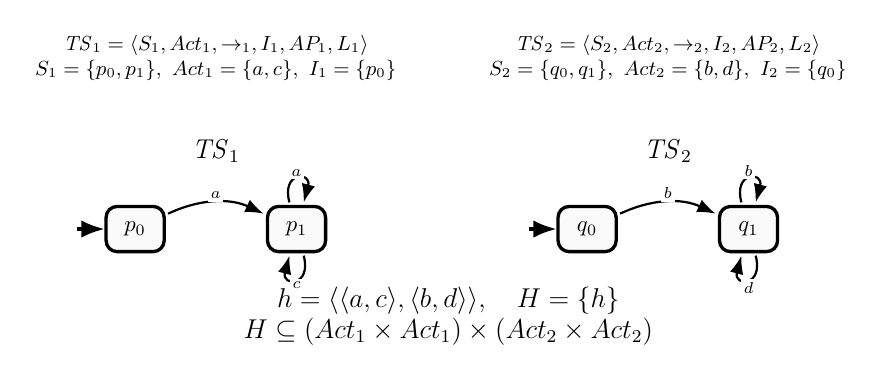
\begin{tikzpicture}[scale=0.82, transform shape]

  \node[align=center, font=\small] at (1.25, 2.65)
    {$\mathit{TS}_1=\langle S_1,Act_1,\to_1,I_1,AP_1,L_1\rangle$\\
     $S_1=\{p_0,p_1\},\ Act_1=\{a,c\},\ I_1=\{p_0\}$};
  \node[align=center, font=\small] at (8.25, 2.65)
    {$\mathit{TS}_2=\langle S_2,Act_2,\to_2,I_2,AP_2,L_2\rangle$\\
     $S_2=\{q_0,q_1\},\ Act_2=\{b,d\},\ I_2=\{q_0\}$};

  \begin{scope}[shift={(0,0)}]
    \node[font=\bfseries\large] at (1.25, 1.2) {$\mathit{TS}_1$};
    \node[nodebox] (p0) at (0,0)   {$p_0$};
    \node[nodebox] (p1) at (2.5,0) {$p_1$};
    \initarrow{(-0.9,0)}{p0.west}
    \draw[edge, bend left=25] (p0) to node[labelbox,above] {$a$} (p1);
    \draw[edge, loop above, looseness=7] (p1) to node[labelbox] {$a$} (p1);
    \draw[edge, loop below, looseness=7] (p1) to node[labelbox] {$c$} (p1);
  \end{scope}

  \node[align=center, font=\large] at (4.85, -1.35)
    {$h=\langle\langle a,c\rangle,\langle b,d\rangle\rangle,\quad H=\{h\}$\\
     $H\subseteq (Act_1\times Act_1)\times(Act_2\times Act_2)$};

  \begin{scope}[shift={(7,0)}]
    \node[font=\bfseries\large] at (1.25, 1.2) {$\mathit{TS}_2$};
    \node[nodebox] (q0) at (0,0)   {$q_0$};
    \node[nodebox] (q1) at (2.5,0) {$q_1$};
    \initarrow{(-0.9,0)}{q0.west}
    \draw[edge, bend left=25] (q0) to node[labelbox,above] {$b$} (q1);
    \draw[edge, loop above, looseness=7] (q1) to node[labelbox] {$b$} (q1);
    \draw[edge, loop below, looseness=7] (q1) to node[labelbox] {$d$} (q1);
  \end{scope}

\end{tikzpicture}
\end{document}
